\section{Pruebas.}

Para verificar el correcto funcionamiento del plugin se realizan diferentes pruebas de exportación de diferentes grados de dificultad. Las primeras pruebas sencillas consisten en la exportación del contenido de ficheros DWG con contenidos básicos:

\begin{itemize}

\item{Fichero con una o varias líneas.}
\item{Fichero con una polilínea}
\item{Fichero con varias polilíneas}
\item{Fichero con un arco}
\item{Fichero con varios arcos}
\item{Fichero combinando todos los elementos anteriores en una sola capa.}
\item{Fichero combinando todos los elementos anteriores en varias capas.}

\end{itemize}

Los resultados de estas pruebas son satisfactorios.

En una segunda fase se obtiene a través del distribuidor de AutoCAD varios ejemplos de ficheros de complejidad media con combinaciones de capas y objetos más complejos.

Los resultados de estas pruebas también son satisfactorios. 

Superados los dos primeros conjuntos de pruebas, se procede a probar con uno de los ficheros originales, utilizados en \cite{Miguel-Munoz}, que se ha establecido como la prueba de validación y verificación del correcto funcionamiento del proceso de exportación. 

En una primera prueba se trata el fichero original reducido, con pocas capas y pocos elementos gráficos. Los resultados son totalmente satisfactorios. A continuación puede verse una captura de pantalla del módulo de visualización \cite{Luis-Fernandez-SSII} realizado por otro alumno que se alimenta del fichero XML generado por el plugin. También se muestra para poder validar el resultado final, el fichero original DWG mostrado por la aplicación AutoCAD.

\begin{figure}[H]
\begin{center}
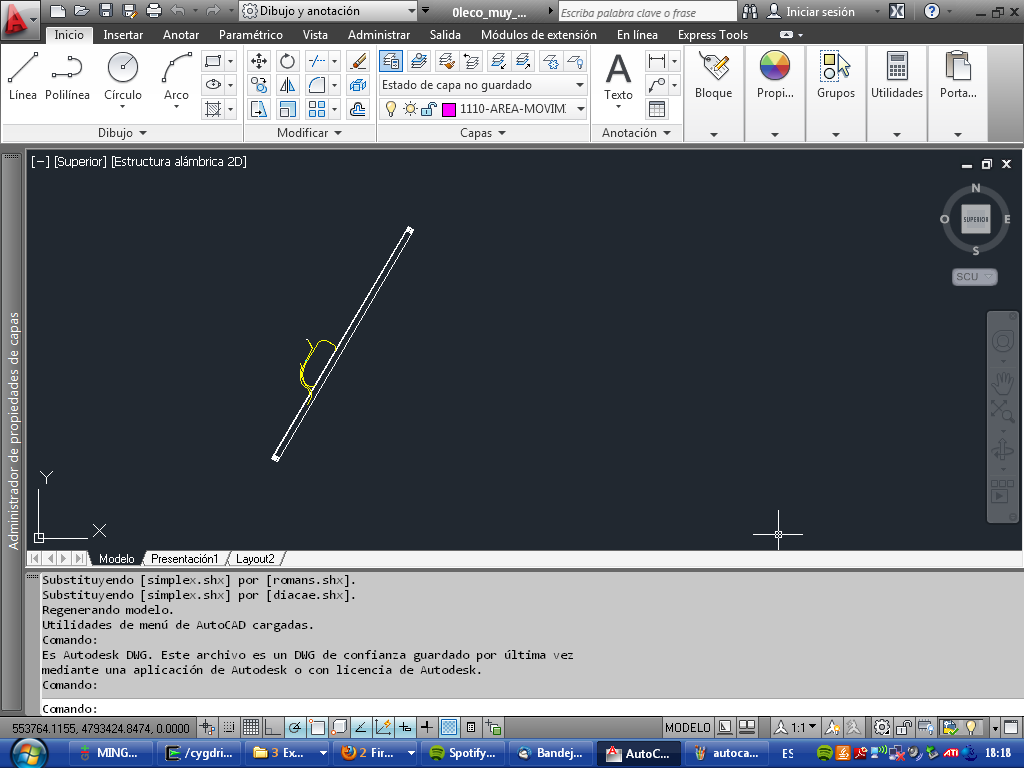
\includegraphics[width=0.8\textwidth]{imgs/autocad2}
\caption{Aplicación AutoCAD mostrando fichero DWG.}
\end{center}
\end{figure}

\begin{figure}[H]
\begin{center}
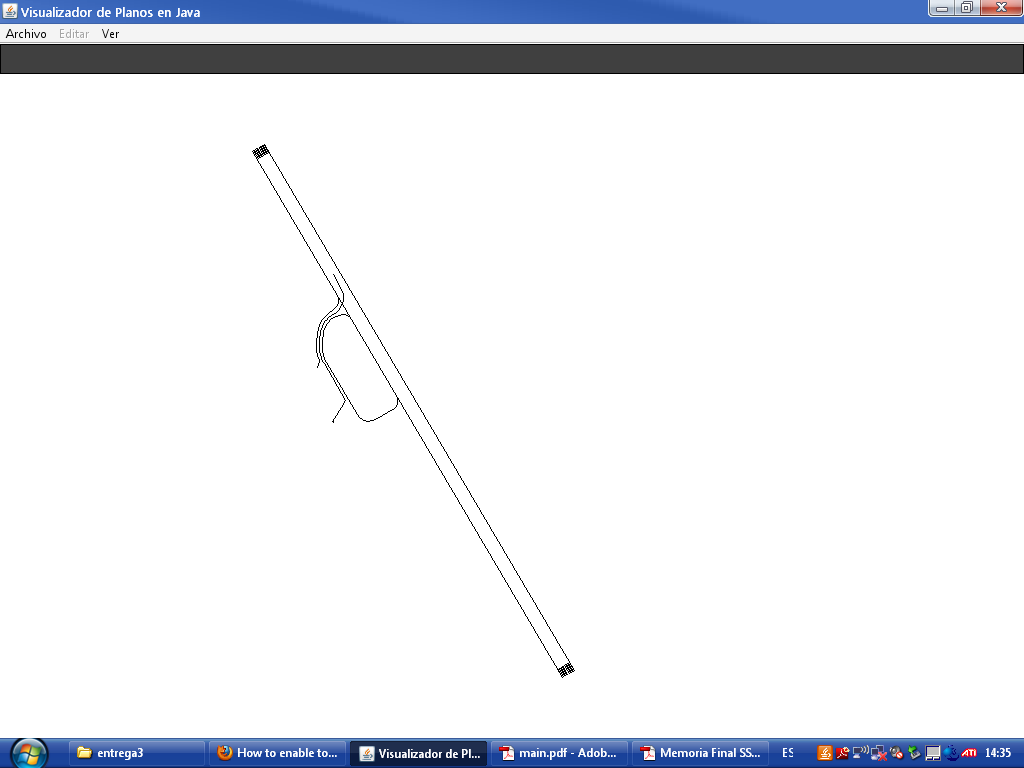
\includegraphics[width=0.8\textwidth]{imgs/ejemplo_salida}
\caption{Módulo visualizador mostrando el contenido del fichero DWG a partir del XML de intercambio \cite{Luis-Fernandez-SSII}.}
\end{center}
\end{figure}

En una segunda prueba se trata el fichero original completo. Los resultados son también totalmente satisfactorios. A continuación puede verse ambas capturas de pantallas:

\begin{figure}[H]
\begin{center}
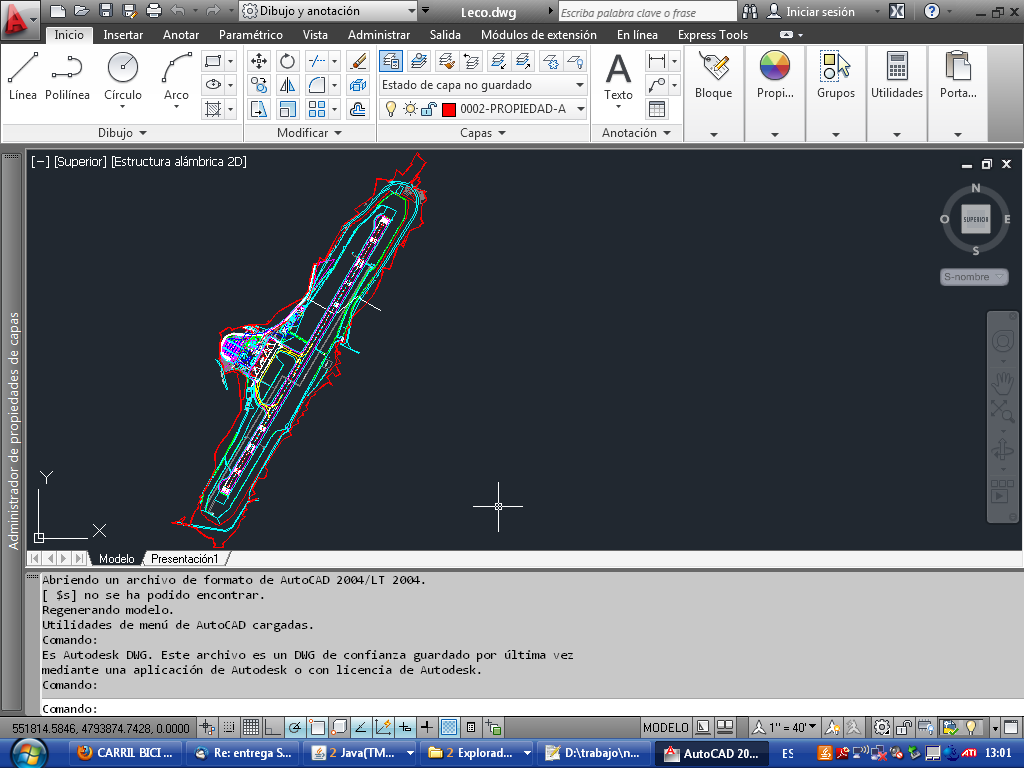
\includegraphics[width=0.8\textwidth]{imgs/autocadleco}
\caption{Aplicación AutoCAD mostrando fichero DWG.}
\end{center}
\end{figure}

\begin{figure}[H]
\begin{center}
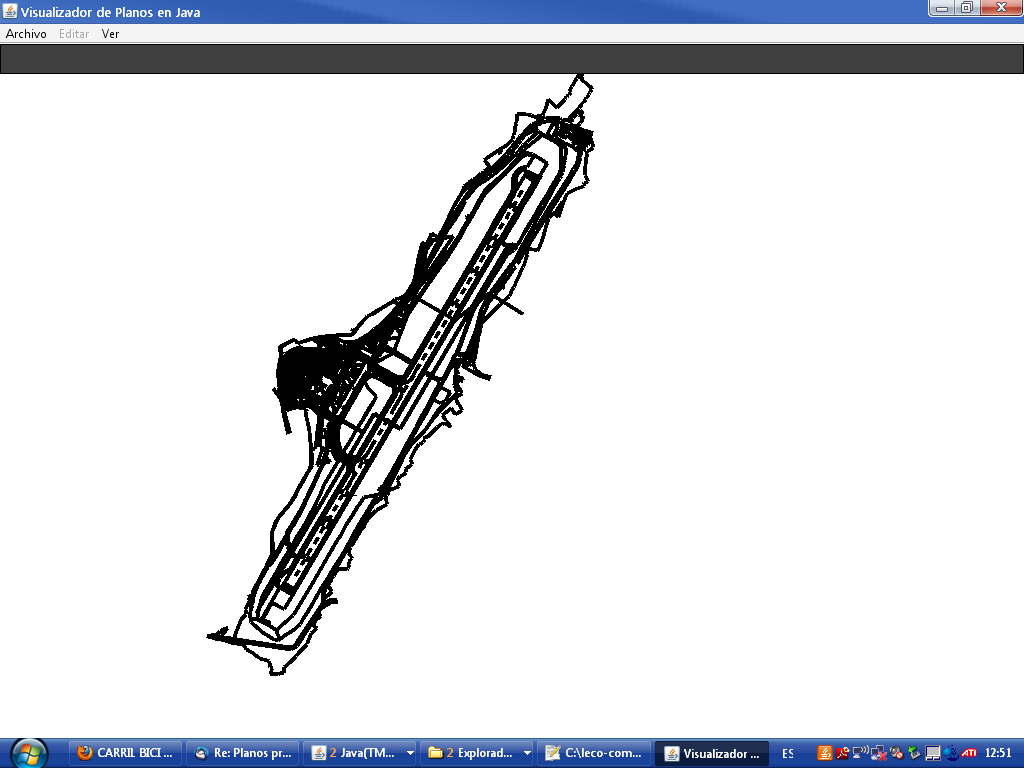
\includegraphics[width=0.8\textwidth]{imgs/ejemplo_salida_2}
\caption{Módulo visualizador mostrando el contenido del fichero DWG a partir del XML de intercambio \cite{Luis-Fernandez-SSII}.}
\end{center}
\end{figure}

En una última fase de pruebas se quiere verificar la consistencia del proceso ante ficheros muy complejos. Se obtiene a través del distribuidor de AutoCAD dos ejemplos de ficheros del diseño de una planta de un edificio nuevo con miles de objetos de distintos tipos en su interior y gran cantidad de capas. 

En esta última fase los resultados son también satisfactorios completándose correctamente la fase de exportación en un tiempo bastante reducido.

Por tanto, tras todas estas pruebas, puede considerarse verificado el correcto funcionamiento del plugin y la consistencia del mismo. A pesar de las pruebas satisfactorias, el proceso de selección de capas puede mejorarse desde el punto de vista de la usabilidad. Funciona correctamente pero podría facilitarse la tarea al usuario a través de algún mecanismo alternativo. Estas posibilidades se describen en el apartado líneas futuras de este documento.

